\documentclass[Report.tex]{subfiles}
\begin{document}

\chapter{Software Architecture}
\section{Architecture pattern}
The application follows the Model-View-Controller (MVC) software architectural pattern, as is currently common with systems that have an emphasis on interactivity via a graphical user interface. MVC has its origins in Smalltalk applications built in the 1980s that SMALLTALK HISTORY

\noindent Figure X shows how the elements of the project align with MVC. The user interacts with elements of the view, in this case a text input form and a graphical button for submission of input to the application. The view specifies the routes through which the data is sent and displayed, as well as the templates for organisation of page content\cite{mozilla_mvc}. The controller receives the input through the web framework and calls functions within the model that can retrieve relevant data based on the search term.  After the data processing is complete, it is sent from the controller to the view to generate output for the user. \newline

\begin{figure}[h!]
	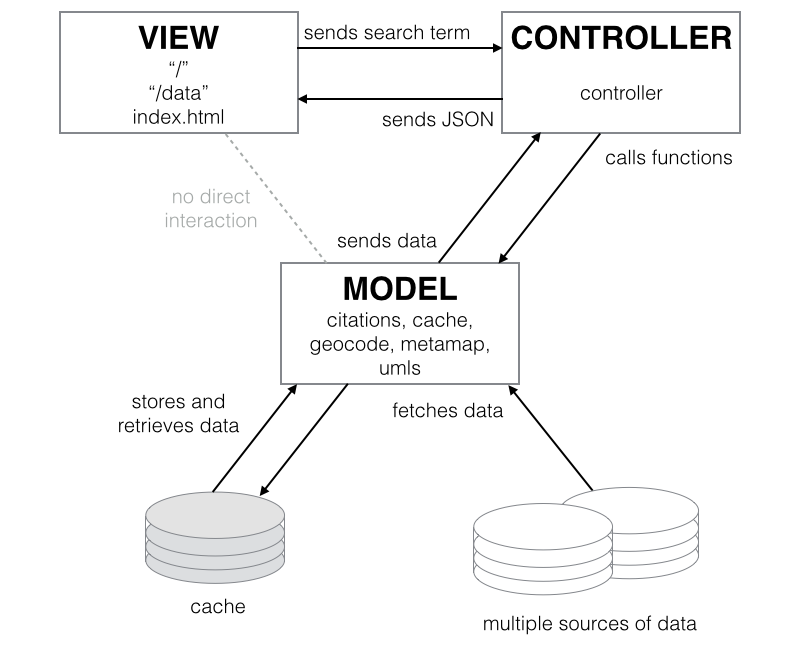
\includegraphics[width=\textwidth]{../lib/images/mvc.png}
	\label{fig:mvc}
	\caption{Diagram to demonstrate fit of the project with the Model-View-Controller software architecture pattern. The routes and HTML template are listed in the View box and the relevant Python modules are listed in the Controller and Model boxes. Each core interaction between the components of the application are displayed next to the directional arrow. The number of data stores are not representative.}
\end{figure}

\noindent The model was focused upon during the development phase of this project, as the efficacy of the view is highly dependent on the quality of the data retrieval and manipulation. 

\section{Application flow}
One of the main challenges of the project was to integrate the various programming languages and technologies required along the pipeline, that are each suited to their specific task but not immediately compatible with one another. Figure X outlines the flow of the application and the key technologies used for each stage. The details of each component will be explored in the next section, Implementation.

\begin{figure}[h!]
	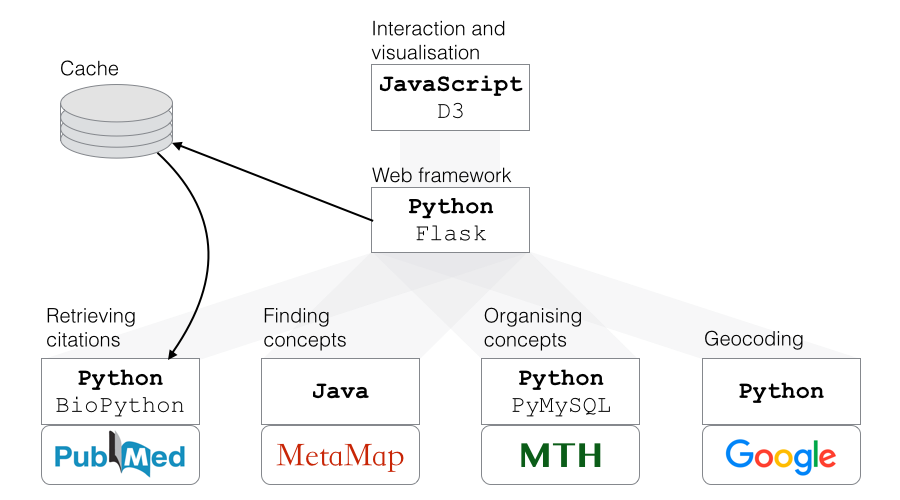
\includegraphics[width=\textwidth]{../lib/images/flow.png}
	\label{fig:flow}
	\caption{Schematic of the key processes of the system, as explained in the text.}
\end{figure}

\begin{enumerate}
\item{\textbf{Interaction of the user with the browser}} 
\newline The client side of the web application is presented in a modern browser. A text field is available upon loading of the web page for the user to enter their search term into.
\item{\textbf{Routing via the Flask web framework}}
\newline CHANGE Search term goes in via javascript, causes GET request from JS to server via '/data' route. This calls a function that launches the pipeline of data retrieval and manipulation.
\item{\textbf{Retrieving information from papers PubMed}}
\newline The PubMed IDs (PMID) of up to 20 papers are retrieved from PubMed via a BioPython function\cite{biopython}. First, a MongoDB cache is queried for any documents with the same PMIDs. Otherwise, the entry is fetched from PubMed using the unique PMID as a reference.
\item{\textbf{Searching the MongoDB cache}}
\newline As mentioned above, a cache has been implemented to reduce the overhead of the numerous HTTP requests and thus improve performance. Each document in the database includes all data as retrieved from PubMed, as well as the MetaMap concepts and Google place IDs found for each paper when initially found and processed. These documents require additional formatting before sending to the client.
\item{\textbf{Extracting medical concepts from papers}}
\newline The abstract, MeSH headings, and author keyword fields of PubMed entries are utilised in order to associate useful, semantically categorised terms with each paper. These are submitted to a service called MetaMap via the Semantic Knowledge Representation (SKR) Java Web API which returns a list of formatted concepts and their Concept Unique Identifiers (CUI).
\item{\textbf{Organising concepts into a semantic hierarchy}}
\newline A local copy of the MetaThesaurus set of vocabularies, organised into a database subset compatible with MySQL, is queried for the CUIs as found in the previous step. There is a 1:1 relationship between each CUI and one Semantic Type, which is returned to inform the visualisation of gross hierarchies. To achieve a more granular representation, a direct parent is also retrieved.
\item{\textbf{Assigning locations to affiliate addresses}}
\newline Addresses as listed in the 'affiliation information' section are formatted to improve success rates, and then sent to the Google Places API to retrieve a result detailing the geographical coordinates of the most likely result. Place IDs are used to fetch coordinates for cached data.
\item{\textbf{Adding new documents to the cache}}
\newline PubMed records are inserted into MongoDB, along with a lists of MetaMap concepts and place IDs for fast repeated retrieval.
\item{\textbf{Data visualisation}}
\newline Data gained from the distinct sources are combined and formatted into Python dicts to send as JSON-formatted data to the client. The Google Map and D3 canvas are updated to reflect the semantic and geographical information representing the data.
\end{enumerate}

\end{document}